\documentclass[dvipsnames]{scrartcl}

\usepackage[margin=2.5cm]{geometry}

\makeatletter
\DeclareOldFontCommand{\rm}{\normalfont\rmfamily}{\mathrm}
\DeclareOldFontCommand{\sf}{\normalfont\sffamily}{\mathsf}
\DeclareOldFontCommand{\tt}{\normalfont\ttfamily}{\mathtt}
\DeclareOldFontCommand{\bf}{\normalfont\bfseries}{\mathbf}
\DeclareOldFontCommand{\it}{\normalfont\itshape}{\mathit}
\DeclareOldFontCommand{\sl}{\normalfont\slshape}{\@nomath\sl}
\DeclareOldFontCommand{\sc}{\normalfont\scshape}{\@nomath\sc}
\makeatother

\usepackage[dvipsnames]{xcolor}
\usepackage{tikz}

\usepackage{cmap} % allows copying math symbols from generated PDF
%\usepackage[only,grbassign]{stmaryrd}

\sloppy

\usepackage{hyperref} 
\usepackage{graphicx}

\usepackage{etoolbox}
\newbool{colored}
\boolfalse{colored}
\newbool{ascii}
\IfFileExists{./ascii}{\booltrue{ascii}}{\boolfalse{ascii}}

\usepackage{subcaption}
\usepackage{xspace}
\usepackage{booktabs}
\usepackage{enumitem}
\usepackage{numprint}
\usepackage{multirow}
\usepackage{xcolor}
\usepackage{todonotes}
\setuptodonotes{inline}

\input{graphblas-commands}
\usetikzlibrary{matrix,arrows,decorations.pathmorphing}
\begin{document}


\begin{figure}
  \centering
  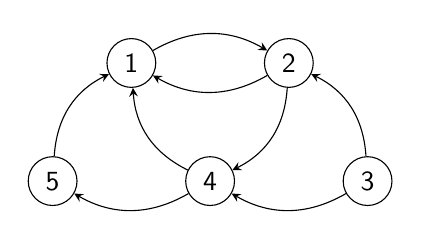
\begin{tikzpicture}[-stealth,align=center,every node/.style={circle, draw}]
      \sf % use sans-serif font
      \node[] at (1, 1.5) (V1) {1};
      \node[] at (3, 1.5) (V2) {2};
      \node[] at (4, 0) (V3) {3};
      \node[] at (2, 0) (V4) {4};
      \node[] at (0, 0) (V5) {5};
      \draw (V1) to [bend left] (V2);
      \draw (V2) to [bend left] (V1);
      \draw (V2) to [bend left] (V4);
      \draw (V3) to [bend right] (V2);
      \draw (V3) to [bend left] (V4);
      \draw (V4) to [bend left] (V1);
      \draw (V4) to [bend left] (V5);
      \draw (V5) to [bend left] (V1);


  \end{tikzpicture}
  \caption{Example directed graph.}
\end{figure}

%%%%%%%%%%%%%%%%%%%%%%%%%%%%%%%%%%%%%%%%%%%%%%%%%%%%%%%%%%%%%%%%%%%%%%%%%%%%%%%%
%%%%%%%%%%%%%%%%%%%%%%%%%%%%%%%%%%%%%%%%%%%%%%%%%%%%%%%%%%%%%%%%%%%%%%%%%%%%%%%%
%%%%%%%%%%%%%%%%%%%%%%%%%%%%%%%%%%%%%%%%%%%%%%%%%%%%%%%%%%%%%%%%%%%%%%%%%%%%%%%%

\newcommand{\myunit}{0.95cm}

\tikzset{
    node style sp/.style={draw,circle,minimum size=\myunit},
    node style ge/.style={circle,minimum size=\myunit},
%    arrow style addition/.style={midway,sloped,fill=white},
%    arrow style multiplication/.style={draw,sloped,midway,fill=white},
    arrow style addition/.style={midway,fill=white,inner sep=1pt},
    arrow style multiplication/.style={draw,midway,fill=white},
}

\begin{figure}
\centering
\begin{tikzpicture}[>=latex]
% 
\matrix (f) [matrix of math nodes,%
              nodes = {node style ge},%
              left delimiter  = {[},%
              right delimiter = {]}] at (0,3)
{%
|[node style sp,RoyalBlue]| 0 &
|[node style sp,RoyalBlue]| 1 &
|[node style sp,RoyalBlue]| 0 &
|[node style sp,RoyalBlue]| 1 &
|[node style sp,RoyalBlue]| 0 \\
};
\matrix (Ai) [matrix of math nodes,%
              nodes = {node style ge}] at (0,2)
{%
  \sf 1 & \sf 2 & \sf 3 & \sf 4 & \sf 5\\
};

\matrix (A) [matrix of math nodes,%
              nodes = {node style ge},%
              left delimiter  ={[},%
              right delimiter ={]}] at (6*\myunit,7*\myunit)
{%
  |[node style sp,RoyalBlue]| 0 & 1 & 0 & 0 & 0 \\
  |[node style sp,RoyalBlue]| 1 & 0 & 0 & 1 & 0 \\
  |[node style sp,RoyalBlue]| 0 & 1 & 0 & 1 & 0 \\
  |[node style sp,RoyalBlue]| 1 & 0 & 0 & 0 & 1 \\
  |[node style sp,RoyalBlue]| 1 & 0 & 0 & 0 & 0 \\
};
\matrix (Bi) [matrix of math nodes,%
              nodes = {node style ge}] at (9.5*\myunit,7*\myunit)
{%
  \sf 1 \\
  \sf 2 \\
  \sf 3 \\
  \sf 4 \\
  \sf 5 \\
};
\matrix (n) [matrix of math nodes,%
              nodes = {node style ge},%
              left delimiter  = {[},%
              right delimiter = {]}] at (6*\myunit,3)
{%
|[node style sp,RoyalBlue]| \tt 2 & \tt 0 & \tt 0 & \tt 1 & \tt 1 \\
};
\matrix (Ci) [matrix of math nodes,%
              nodes = {node style ge}] at (6*\myunit,2)
{%
  \sf 1 & \sf 2 & \sf 3 & \sf 4 & \sf 5\\
};

\tiny
\draw[-,RoyalBlue](f-1-1) to[in=180,out=90] node[arrow style multiplication] (x) {$0 \times 0 = 0$} (A-1-1);
\draw[-,RoyalBlue](f-1-2) to[in=180,out=90] node[arrow style multiplication] (y) {$1 \times 1 = 1$} (A-2-1);
\draw[-,RoyalBlue](f-1-3) to[in=180,out=90] node[arrow style multiplication] (z) {$0 \times 0 = 0$} (A-3-1);
\draw[-,RoyalBlue](f-1-4) to[in=180,out=90] node[arrow style multiplication] (w) {$1 \times 1 = 1$} (A-4-1);
\draw[-,RoyalBlue](f-1-5) to[in=180,out=90] node[arrow style multiplication] (v) {$0 \times 1 = 0$} (A-5-1);
\draw[RoyalBlue,->] (x)
  to node[arrow style addition] {\tiny $+$} (y)%
  to node[arrow style addition] {\tiny $+$} (z)%
  to node[arrow style addition] {\tiny $+$} (w)%
  to node[arrow style addition] {\tiny $+$} (v)%
  to (n-1-1.north west) ;

\end{tikzpicture}
\caption{Dense vector-matrix multiplication $\grbv{f} \grbm{A}$ on the conventional \textcolor{RoyalBlue}{$\grbsemiringops{+}{\times}$} semiring.}
\end{figure}

%%%%%%%%%%%%%%%%%%%%%%%%%%%%%%%%%%%%%%%%%%%%%%%%%%%%%%%%%%%%%%%%%%%%%%%%%%%%%%%%
%%%%%%%%%%%%%%%%%%%%%%%%%%%%%%%%%%%%%%%%%%%%%%%%%%%%%%%%%%%%%%%%%%%%%%%%%%%%%%%%
%%%%%%%%%%%%%%%%%%%%%%%%%%%%%%%%%%%%%%%%%%%%%%%%%%%%%%%%%%%%%%%%%%%%%%%%%%%%%%%%

\begin{figure}
\centering
\begin{tikzpicture}[>=latex]
% 
\matrix (f) [matrix of math nodes,%
              nodes = {node style ge},%
              left delimiter  = {[},%
              right delimiter = {]}] at (0,3)
{%
  \phantom{1} & |[node style sp,RoyalBlue]| 1 & \phantom{1} & |[node style sp,RoyalBlue]| 1 & \phantom{1} \\
};
\matrix (Ai) [matrix of math nodes,%
              nodes = {node style ge}] at (0,2)
{%
  \sf 1 & \sf 2 & \sf 3 & \sf 4 & \sf 5\\
};

\matrix (A) [matrix of math nodes,%
              nodes = {node style ge},%
              left delimiter  ={[},%
              right delimiter ={]}] at (6*\myunit,7*\myunit)
{%
                        &     1 & \vphantom{.} &       &       \\
|[node style sp,RoyalBlue]|     1 &       &        &     1 &       \\
                        &     1 &        &     1 &       \\
|[node style sp,RoyalBlue]|     1 &       &        &       &     1 \\
                      1 &       &        &       &       \\
};
\matrix (Bi) [matrix of math nodes,%
              nodes = {node style ge}] at (9.5*\myunit,7*\myunit)
{%
  \sf 1 \\
  \sf 2 \\
  \sf 3 \\
  \sf 4 \\
  \sf 5 \\
};
%
\matrix (n) [matrix of math nodes,%
              nodes = {node style ge},%
              left delimiter  = {[},%
              right delimiter = {]}] at (6*\myunit,3)
{%
|[node style sp,RoyalBlue]| \tt 2 & \ & \ & \tt 1 & \tt 1 \\
};
\matrix (Ci) [matrix of math nodes,%
              nodes = {node style ge}] at (6*\myunit,2)
{%
  \sf 1 & \sf 2 & \sf 3 & \sf 4 & \sf 5\\
};

\draw[-,RoyalBlue](f-1-2) to[in=180,out=90] node[arrow style multiplication] (x) {$1 \times 1 = \tt 1$} (A-2-1);
\draw[-,RoyalBlue](f-1-4) to[in=180,out=90] node[arrow style multiplication] (y) {$1 \times 1 = \tt 1$} (A-4-1);
\draw[RoyalBlue,->] (x)
  to node[arrow style addition] {$+$} (y)%
  to (n-1-1.north west) ;

\end{tikzpicture}
\caption{Sparse vector-matrix multiplication $\grbv{f} \grbm{A}$ on the conventional \textcolor{RoyalBlue}{$\grbsemiringops{+}{\times}$} semiring.}
\end{figure}

%%%%%%%%%%%%%%%%%%%%%%%%%%%%%%%%%%%%%%%%%%%%%%%%%%%%%%%%%%%%%%%%%%%%%%%%%%%%%%%%
%%%%%%%%%%%%%%%%%%%%%%%%%%%%%%%%%%%%%%%%%%%%%%%%%%%%%%%%%%%%%%%%%%%%%%%%%%%%%%%%
%%%%%%%%%%%%%%%%%%%%%%%%%%%%%%%%%%%%%%%%%%%%%%%%%%%%%%%%%%%%%%%%%%%%%%%%%%%%%%%%

\begin{figure}
\centering
\begin{tikzpicture}[>=latex]
% 
\matrix (f) [matrix of math nodes,%
              nodes = {node style ge},%
              left delimiter  = {[},%
              right delimiter = {]}] at (0,3)
{%
  \phantom{\grbT} & |[node style sp,OliveGreen]| \grbT & \phantom{\grbT} & |[node style sp,OliveGreen]| \grbT & \phantom{\grbT} \\
};
\matrix (Ai) [matrix of math nodes,%
              nodes = {node style ge}] at (0,2)
{%
  \sf 1 & \sf 2 & \sf 3 & \sf 4 & \sf 5\\
};

\matrix (A) [matrix of math nodes,%
              nodes = {node style ge},%
              left delimiter  ={[},%
              right delimiter ={]}] at (6*\myunit,7*\myunit)
{%
                        & \grbT & \vphantom{.} &       &       \\
|[node style sp,OliveGreen]| \grbT &       &        & \grbT &       \\
                        & \grbT &        & \grbT &       \\
|[node style sp,OliveGreen]| \grbT &       &        &       & \grbT \\
                  \grbT &       &        &       &       \\
};
\matrix (Bi) [matrix of math nodes,%
              nodes = {node style ge}] at (9.5*\myunit,7*\myunit)
{%
  \sf 1 \\
  \sf 2 \\
  \sf 3 \\
  \sf 4 \\
  \sf 5 \\
};
%
\matrix (n) [matrix of math nodes,%
              nodes = {node style ge},%
              left delimiter  = {[},%
              right delimiter = {]}] at (6*\myunit,3)
{%
|[node style sp,OliveGreen]| \tt \grbT & \ & \ & \tt \grbT & \tt \grbT \\
};
\matrix (Ci) [matrix of math nodes,%
              nodes = {node style ge}] at (6*\myunit,2)
{%
  \sf 1 & \sf 2 & \sf 3 & \sf 4 & \sf 5\\
};

\draw[-,OliveGreen](f-1-2) to[in=180,out=90] node[arrow style multiplication] (x) {$\grbT \, \grbland \, \grbT = \grbT$} (A-2-1);
\draw[-,OliveGreen](f-1-4) to[in=180,out=90] node[arrow style multiplication] (y) {$\grbT \, \grbland \, \grbT = \grbT$} (A-4-1);
\draw[OliveGreen,->] (x)
  to node[arrow style addition] {$\grblor$} (y)%
  to (n-1-1.north west) ;

\end{tikzpicture}
\caption{Sparse vector-matrix multiplication $\grbv{f} \grbm{A}$ on the \textcolor{OliveGreen}{$\grblorland$} ($\vee.\wedge$) semiring.}
\end{figure}

%%%%%%%%%%%%%%%%%%%%%%%%%%%%%%%%%%%%%%%%%%%%%%%%%%%%%%%%%%%%%%%%%%%%%%%%%%%%%%%%
%%%%%%%%%%%%%%%%%%%%%%%%%%%%%%%%%%%%%%%%%%%%%%%%%%%%%%%%%%%%%%%%%%%%%%%%%%%%%%%%
%%%%%%%%%%%%%%%%%%%%%%%%%%%%%%%%%%%%%%%%%%%%%%%%%%%%%%%%%%%%%%%%%%%%%%%%%%%%%%%%

\begin{figure}
\centering
\begin{tikzpicture}[>=latex]
% 
\matrix (f) [matrix of math nodes,%
              nodes = {node style ge},%
              left delimiter  = {[},%
              right delimiter = {]}] at (0,3)
{%
  \phantom{\grbT} & |[node style sp,RubineRed]| \grbT & \phantom{\grbT} & |[node style sp,RubineRed]| \grbT & \phantom{\grbT} \\
};
\matrix (Ai) [matrix of math nodes,%
              nodes = {node style ge}] at (0,2)
{%
  \sf 1 & \sf 2 & \sf 3 & \sf 4 & \sf 5\\
};

\matrix (A) [matrix of math nodes,%
              nodes = {node style ge},%
              left delimiter  ={[},%
              right delimiter ={]}] at (6*\myunit,7*\myunit)
{%
                            & \grbT        & \vphantom{.} &       &       \\
|[node style sp,RubineRed]| \grbT &              &              & \grbT &       \\
                            & \grbT        &              & \grbT &       \\
|[node style sp,RubineRed]| \grbT &              &              &       & \grbT \\
                      \grbT &              &              &       &       \\
};
\matrix (Bi) [matrix of math nodes,%
              nodes = {node style ge}] at (9.5*\myunit,7*\myunit)
{%
  \sf 1 \\
  \sf 2 \\
  \sf 3 \\
  \sf 4 \\
  \sf 5 \\
};
%
\matrix (n) [matrix of math nodes,%
              nodes = {node style ge},%
              left delimiter  = {[},%
              right delimiter = {]}] at (6*\myunit,3)
{%
|[node style sp,RubineRed]| \tt \grbT & \ & \ & \tt \grbT & \tt \grbT \\
};
\matrix (Ci) [matrix of math nodes,%
              nodes = {node style ge}] at (6*\myunit,2)
{%
  \sf 1 & \sf 2 & \sf 3 & \sf 4 & \sf 5\\
};

%\draw[-,RubineRed](f-1-2) to[in=180,out=90] node[arrow style multiplication] (x) {$\grbv{f}(2) \, \grbpair \, \grbm{A}(\sf 2, 1) = \grbT$} (A-2-1);
%\draw[-,RubineRed](f-1-4) to[in=180,out=90] node[arrow style multiplication] (y) {$\grbv{f}(4) \, \grbpair \, \grbm{A}(\sf 4, 1) = \grbT$} (A-4-1);
\draw[-,RubineRed](f-1-2) to[in=180,out=90] node[arrow style multiplication] (x) {$\grbdontcare \, \grbpair \, \grbdontcare = \grbT$} (A-2-1);
\draw[-,RubineRed](f-1-4) to[in=180,out=90] node[arrow style multiplication] (y) {$\grbdontcare \, \grbpair \, \grbdontcare = \grbT$} (A-4-1);
\draw[RubineRed,->] (x)
  to node[arrow style addition] {$\grbany$} (y)%
  to (n-1-1.north west) ;

\end{tikzpicture}
\caption{Sparse vector-matrix multiplication $\grbv{f} \grbm{A}$ on the \textcolor{RubineRed}{$\grbanypair$} semiring (currently only available in \gxb). The \emph{don't-care} values are denoted with the $\grbdontcare$ symbol.}
\end{figure}

%%%%%%%%%%%%%%%%%%%%%%%%%%%%%%%%%%%%%%%%%%%%%%%%%%%%%%%%%%%%%%%%%%%%%%%%%%%%%%%%
%%%%%%%%%%%%%%%%%%%%%%%%%%%%%%%%%%%%%%%%%%%%%%%%%%%%%%%%%%%%%%%%%%%%%%%%%%%%%%%%
%%%%%%%%%%%%%%%%%%%%%%%%%%%%%%%%%%%%%%%%%%%%%%%%%%%%%%%%%%%%%%%%%%%%%%%%%%%%%%%%

\begin{figure}
  \centering
  \begin{tikzpicture}[>=latex]
  % 
  \matrix (f) [matrix of math nodes,%
                nodes = {node style ge},%
                left delimiter  = {[},%
                right delimiter = {]}] at (0,3)
  {%
    \phantom{\grbT} & |[node style sp,Plum]| \grbT & \phantom{\grbT} & |[node style sp,Plum]| \grbT & \phantom{\grbT} \\
  };
  \matrix (Ai) [matrix of math nodes,%
                nodes = {node style ge}] at (0,2)
  {%
    \sf 1 & \sf 2 & \sf 3 & \sf 4 & \sf 5\\
  };
  
  \matrix (A) [matrix of math nodes,%
                nodes = {node style ge},%
                left delimiter  ={[},%
                right delimiter ={]}] at (6*\myunit,7*\myunit)
  {%
                            & \grbT & \vphantom{.} &       &       \\
    |[node style sp,Plum]| \grbT &       &        & \grbT &       \\
                            & \grbT &        & \grbT &       \\
    |[node style sp,Plum]| \grbT &       &        &       & \grbT \\
                      \grbT &       &        &       &       \\
  };
  \matrix (Bi) [matrix of math nodes,%
                nodes = {node style ge}] at (9.5*\myunit,7*\myunit)
  {%
    \sf 1 \\
    \sf 2 \\
    \sf 3 \\
    \sf 4 \\
    \sf 5 \\
  };
  
  \matrix (n) [matrix of math nodes,%
                nodes = {node style ge},%
                left delimiter  = {[},%
                right delimiter = {]}] at (6*\myunit,3)
  {%
  |[node style sp,Plum]| \tt 2 & \ & \ & \tt 2 & \tt 4 \\
  };
  \matrix (Ci) [matrix of math nodes,%
                nodes = {node style ge}] at (6*\myunit,2)
  {%
    \sf 1 & \sf 2 & \sf 3 & \sf 4 & \sf 5\\
  };
  
  % les fleches
  \draw[-,Plum](f-1-2) to[in=180,out=90] node[arrow style multiplication] (x) {$\grbv{f}(2) \, \grbsecondione \, \grbm{A}(\sf 2, 1) = \tt 2$} (A-2-1);
  \draw[-,Plum](f-1-4) to[in=180,out=90] node[arrow style multiplication] (y) {$\grbv{f}(4) \, \grbsecondione \, \grbm{A}(\sf 4, 1) = \tt 4$} (A-4-1);
  \draw[Plum,->] (x)
    to node[arrow style addition] {$\grbmin$} (y)%
    to (n-1-1.north west) ;
  
  \end{tikzpicture}
  \caption{Sparse vector-matrix multiplication $\grbv{f} \grbm{A}$ on the \textcolor{Plum}{$\grbminsecondione$} %{$\grbminfirstjone$}
  semiring (only available in \gxb).
  %The $\grbfirstjone$ operator returns the column index of the first operand using 1-based indexing.
  The $\grbsecondione$ operator returns the row index of the element in the second operand using 1-based indexing.
  }
\end{figure}

%%%%%%%%%%%%%%%%%%%%%%%%%%%%%%%%%%%%%%%%%%%%%%%%%%%%%%%%%%%%%%%%%%%%%%%%%%%%%%%%
%%%%%%%%%%%%%%%%%%%%%%%%%%%%%%%%%%%%%%%%%%%%%%%%%%%%%%%%%%%%%%%%%%%%%%%%%%%%%%%%
%%%%%%%%%%%%%%%%%%%%%%%%%%%%%%%%%%%%%%%%%%%%%%%%%%%%%%%%%%%%%%%%%%%%%%%%%%%%%%%%

\begin{figure}
  \centering
  \begin{tikzpicture}[>=latex]
  % 
  \matrix (f) [matrix of math nodes,%
                nodes = {node style ge},%
                left delimiter  = {[},%
                right delimiter = {]}] at (0,3)
  {%
    \phantom{\grbT} & |[node style sp,Plum]| \grbT & \phantom{\grbT} & |[node style sp,Plum]| \grbT & \phantom{\grbT} \\
  };
  \matrix (Ai) [matrix of math nodes,%
                nodes = {node style ge}] at (0,2)
  {%
    \sf 1 & \sf 2 & \sf 3 & \sf 4 & \sf 5\\
  };
  
  \matrix (A) [matrix of math nodes,%
                nodes = {node style ge},%
                left delimiter  ={[},%
                right delimiter ={]}] at (6*\myunit,7*\myunit)
  {%
                            & \grbT & \vphantom{.} &       &       \\
    |[node style sp,Plum]| \grbT &       &        & \grbT &       \\
                            & \grbT &        & \grbT &       \\
    |[node style sp,Plum]| \grbT &       &        &       & \grbT \\
                      \grbT &       &        &       &       \\
  };
  \matrix (Bi) [matrix of math nodes,%
                nodes = {node style ge}] at (9.5*\myunit,7*\myunit)
  {%
    \sf 1 \\
    \sf 2 \\
    \sf 3 \\
    \sf 4 \\
    \sf 5 \\
  };
  
  \matrix (n) [matrix of math nodes,%
                nodes = {node style ge},%
                left delimiter  = {[},%
                right delimiter = {]}] at (6*\myunit,3)
  {%
  |[node style sp,Plum]| \tt 2 & \ & \ & \tt 2 & \tt 4 \\
  };
  \matrix (Ci) [matrix of math nodes,%
                nodes = {node style ge}] at (6*\myunit,2)
  {%
    \sf 1 & \sf 2 & \sf 3 & \sf 4 & \sf 5\\
  };
  
    % \draw[-,Plum](f-1-2) to[in=180,out=90] node[arrow style multiplication] (x) {$\grbv{f}(2) \, \grbsecondione \, \grbm{A}(\sf 2, 1) = \tt 2$} (A-2-1);
  % \draw[-,Plum](f-1-4) to[in=180,out=90] node[arrow style multiplication] (y) {$\grbv{f}(4) \, \grbsecondione \, \grbm{A}(\sf 4, 1) = \tt 4$} (A-4-1);
  % \draw[-,Plum](f-1-2) to[in=180,out=90] node[arrow style multiplication] (x) {$\grbdontcare \, \grbsecondione \, \grbdontcare = \tt 2$} (A-2-1);
  % \draw[-,Plum](f-1-4) to[in=180,out=90] node[arrow style multiplication] (y) {$\grbdontcare \, \grbsecondione \, \grbdontcare = \tt 4$} (A-4-1);
  \draw[-,Plum](f-1-2) to[in=180,out=90] node[arrow style multiplication] (x) {$\grbsecondione(\grbdontcare, \grbdontcare) = \tt 2$} (A-2-1);
  \draw[-,Plum](f-1-4) to[in=180,out=90] node[arrow style multiplication] (y) {$\grbsecondione(\grbdontcare, \grbdontcare) = \tt 4$} (A-4-1);
  \draw[Plum,->] (x)
    to node[arrow style addition] {$\grbmin$} (y)%
    to (n-1-1.north west) ;
  
  \end{tikzpicture}
  \caption{Sparse vector-matrix multiplication $\grbv{f} \grbm{A}$ on the \textcolor{Plum}{$\grbminsecondione$} %{$\grbminfirstjone$}
  semiring (only available in \gxb).
  %The $\grbfirstjone$ operator returns the column index of the first operand using 1-based indexing.
  The $\grbsecondione$ operator returns the row index of the element in the second operand using 1-based indexing. This figure uses \emph{don't-care} values ($\grbdontcare$).
  }
\end{figure}


\end{document}
